
\tikzstyle{boxpackage} = [rectangle, rounded corners, minimum width=0.7cm, minimum height=0.6cm,text centered, draw=black, font=\footnotesize]

% Mathematics
\begin{frame}[fragile]
 \frametitle{Mathematics}
 \begin{block}{} 
  \begin{center}
   \begin{tikzpicture}[node distance=0.7cm, scale=0.5]
    \only<1-3>{
    \node (problem) [boxpackage, fill=\myblue] {Problem};
    }
    \visible<2->{
    \node (model) [boxpackage, below of=problem, yshift = -3em, fill=\myblue] {Mathematical context};
    }
    \only<2-3>{
    \draw[->,thick] (problem) --node[right]{Abstraction} (model);
    }
    \visible<3->{
    \node (solution) [boxpackage, below of=model,yshift = -3em, fill=\myblue] {Solution};    
    \draw[->,thick] (model) --node[right]{Methods} (solution);
    }
    \visible<4->{
    \node (problem1) [boxpackage, fill=\myblue] {Problem};
    \node (problem2) [boxpackage, fill=\myblue, left = of problem1] {Problem};
    \node (problem3) [boxpackage, fill=\myblue, right = of problem1] {Problem};
    \node (dotsleft) [left = of problem2] {$\dots$};
    \node (dotsright) [right = of problem3] {$\dots$};
    \draw[->,thick] (problem1) -- (model);
    \draw[->,thick] (problem2) -- (model);
    \draw[->,thick] (problem3) -- (model);
    \draw[->,thick] (dotsleft) -- (model);
    \draw[->,thick] (dotsright) -- (model);
    }
    \visible<5->{
    \draw[draw=none] (problem1) --node[]{$\simeq$} (problem2);
    \draw[draw=none] (problem3) --node[]{$\simeq$} (problem1);
    \draw[draw=none] (problem3) --node[]{$\simeq$} (dotsright);
    \draw[draw=none] (dotsleft) --node[]{$\simeq$} (problem2);
    }
    \end{tikzpicture}
  \end{center}
 \end{block}
\end{frame}

% Constructive category theory
\begin{frame}[fragile]
 \frametitle{Constructive category theory}
 \begin{block}{} 
  \begin{center}
   \begin{tikzpicture}[node distance=0.7cm, scale=0.6, every node/.style={scale=0.6}]
    \only<1-3>{
    \node (problem) [boxpackage, fill=\myblue] {Mathematical context};
    }
    \visible<2->{
    \node (model) [boxpackage, below of=problem, yshift = -3em, fill=\myblue] {Category};
    }
    \only<2>{
    \draw[->,thick] (problem) --node[right]{Abstraction} (model);
    }
    \visible<6->{
    \node (solution) [boxpackage, below of=model,yshift = -3em, fill=\myblue] {Solution};    
    \draw[->,thick] (model) --node[right]{Constructive category theory} (solution);
    }
    \visible<3->{
    \node (problem1) [boxpackage, fill=\myblue] {Mathematical context};
    \node (problem2) [boxpackage, fill=\myblue, left = of problem1] {Mathematical context};
    \node (problem3) [boxpackage, fill=\myblue, right = of problem1] {Mathematical context};
    \node (dotsleft) [left = of problem2] {$\dots$};
    \node (dotsright) [right = of problem3] {$\dots$};
    \draw[->,thick] (problem1) -- (model);
    \draw[->,thick] (problem2) -- (model);
    \draw[->,thick] (problem3) -- (model);
    \draw[->,thick] (dotsleft) -- (model);
    \draw[->,thick] (dotsright) -- (model);
    }
    \visible<4->{
    \draw[draw=none] (problem1) --node[]{$\simeq$} (problem2);
    \draw[draw=none] (problem3) --node[]{$\simeq$} (problem1);
    \draw[draw=none] (problem3) --node[]{$\simeq$} (dotsright);
    \draw[draw=none] (dotsleft) --node[]{$\simeq$} (problem2);
    }
    \visible<5->{
    \node (problem1n) [boxpackage, fill=\myblue, above = of problem1,xshift=+2.5em] {Problem};
    \node (problem2n) [boxpackage, fill=\myblue, above = of problem2,xshift=+2.5em] {Problem};
    \node (problem3n) [boxpackage, fill=\myblue, above = of problem3,xshift=+2.5em] {Problem};
    \node (problem1m) [boxpackage, fill=\myblue, above = of problem1,xshift=-2.5em] {Problem};
    \node (problem2m) [boxpackage, fill=\myblue, above = of problem2,xshift=-2.5em] {Problem};
    \node (problem3m) [boxpackage, fill=\myblue, above = of problem3,xshift=-2.5em] {Problem};
    \node (dotsleft) [left = of problem2m, xshift = +1em] {$\dots$};
    \node (dotsright) [right = of problem3n, xshift = -1em] {$\dots$};
%     
%     
    \draw[draw=none] (problem1n) --node[]{$\simeq$} (problem1m);
    \draw[draw=none] (problem2n) --node[]{$\simeq$} (problem2m);
    \draw[draw=none] (problem3n) --node[]{$\simeq$} (problem3m);
    
    \draw[draw=none] (problem2m) --node[]{$\simeq$} (problem1n);
    \draw[draw=none] (problem1m) --node[]{$\simeq$} (problem3n);
    \draw[draw=none] (problem2m) --node[]{$\simeq$} (dotsleft);
    \draw[draw=none] (problem3n) --node[]{$\simeq$} (dotsright);
    
    
    \draw[->,thick] (problem1n) -- (problem1);
    \draw[->,thick] (problem1m) -- (problem1);
    \draw[->,thick] (problem2n) -- (problem2);
    \draw[->,thick] (problem2m) -- (problem2);
    \draw[->,thick] (problem3n) -- (problem3);
    \draw[->,thick] (problem3m) -- (problem3);
    \draw[->,thick] (dotsleft) -- (problem2);
    \draw[->,thick] (dotsright) -- (problem3);
    
%     \draw[draw=none] (dotsrightn) --node[]{$\simeq$} (problem1n);
%     \draw[draw=none] (dotsrightn1) --node[]{$\simeq$} (problem3n);
%     \draw[draw=none] (dotsleftn1) --node[]{$\simeq$} (problem2n);
%     \draw[->,thick] (problem1n) -- (problem1);
%     \draw[->,thick] (problem2n) -- (problem2);
%     \draw[->,thick] (problem3n) -- (problem3);
    }
    \end{tikzpicture}
  \end{center}
 \end{block}
\end{frame}

% Abstraction of language
\begin{frame}[fragile]
 \frametitle{Abstraction of language}
 \pause
 \begin{block}{Addition of two numbers:\vphantom{AssemblyC\Gap or Julia} \only<3-5>{Assembly}\only<6-8>{C}\only<9->{\Gap or Julia}}
  \vspace*{-1.5em}
  \begin{overlayarea}{\linewidth}{12\baselineskip}

 \only<2-11>{
 \begin{columns}[onlytextwidth, t]
  \column{0.02\linewidth}
  
  \column{0.40\linewidth}
  \begin{block}{Data type: \texttt{int}}
  \begin{overlayarea}{\linewidth}{8\baselineskip}
\only<4-5>{
\vspace*{-1em}
\assemblyint
}
\only<7-8>{
 \cinteger
}
\only<10-11>{
 \juliacode
}
  \end{overlayarea}
  \end{block}
  \column{0.40\linewidth}
  \begin{block}{Data type: \texttt{float}}
  \begin{overlayarea}{\linewidth}{8\baselineskip}
\only<5>{
  \vspace*{-1em}
\assemblyfloat
}
\only<8>{
\cfloat
}
\only<11>{
 \juliacode
}
 \end{overlayarea}
 \end{block}
 \column{0.02\linewidth}
 \end{columns}
}
\only<12->{
 \begin{columns}
  \column{0.02\linewidth}
  
  \column{0.8\linewidth}
  \vspace{1.5em}
  \begin{block}{Data type: \texttt{int, float}}
  \juliacode
 \end{block}
 \begin{center}
  \visible<13->{High language leads to generic code!}
 \end{center}

 \column{0.02\linewidth}
 \end{columns}
}
 \end{overlayarea}
 \end{block}
\end{frame}

% Abstraction of language
\begin{frame}[fragile]
 \frametitle{Abstraction of language}
 \begin{block}{Computing the intersection of two subobjects}
  \begin{columns}[onlytextwidth, t]
  \column{0.02\linewidth}
  \column{0.40\linewidth}
  \pause
  \begin{block}{Vector spaces\vphantom{Ideals of $\mathbb{Z}$}}
  \begin{overlayarea}{\linewidth}{7\baselineskip}
  $\left\langle v_1, v_2 \right\rangle, \left\langle w_1, w_2 \right\rangle \leq V$:\newline \pause
  Solution of
  \begin{align*}
   & x_1v_1 + x_2 v_2 \\
   = & y_1w_1 +y_2w_2
  \end{align*}
  \end{overlayarea}
  \end{block} \pause
  \column{0.40\linewidth}
  \begin{block}{Ideals of $\mathbb{Z}$\vphantom{Vector spaces}} \pause
  \begin{overlayarea}{\linewidth}{7\baselineskip}
  $\left\langle x\right\rangle$, $\left\langle y\right\rangle \leq \Z:$\newline \pause
  Euclidean algorithm:
  \[
   \left\langle \mathrm{lcm} \left( x,y \right) \right\rangle
  \]
  
  \end{overlayarea}
  \end{block}\pause
  \column{0.02\linewidth}
  \end{columns}
 \begin{center}
 Generic algorithm for both cases? \pause
 \textbf{Category theory!}
 \end{center}
 \end{block}
\end{frame}

% Category theory as programming language
\begin{frame}
\frametitle{Category theory as programming language}
 \begin{block}{Category theory} \pause
 \begin{itemize}
  \item abstracts mathematical structures \pause
  \item defines a \textit{language} to formulate theorems and algorithms for different structures \textit{at the same time}\pause
 \end{itemize} 
 \end{block}
 \begin{block}{\CapPkg\ - Categories, Algorithms, Programming}
  \begin{columns}[onlytextwidth, t]
   \column{0.02\linewidth}
   \column{0.2\linewidth}
   \vspace{0.1em}
 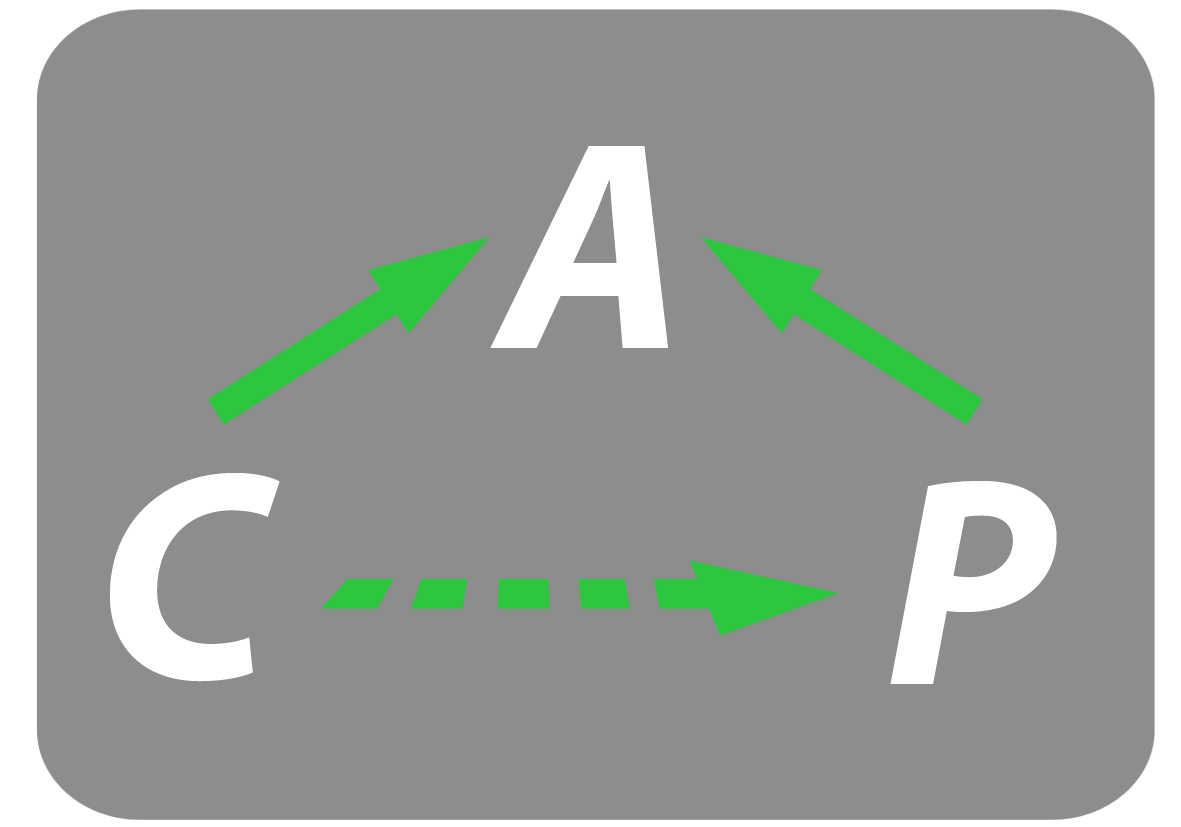
\includegraphics[width=\textwidth,height=0.8\textwidth]{Logo_CAPtrans.png} \pause
 \column{0.7\linewidth}
   \begin{center}
   \hspace{2em}\CapPkg implements a \newline \textbf{categorical programming language}
   \end{center}
  \column{0.02\linewidth}
  \end{columns}
 \end{block}
\end{frame}

% Categories
\begin{frame}[fragile]
 \frametitle{Categories}
 \begin{block}{Definition}
  A category $\mathcal{A}$ contains the following data:
  \pause
  \begin{itemize}
   \item $\Obj_\mathcal{A}$
   \visible<3->{
   \item $\Hom_\mathcal{A}( A, B )$}
   \visible<6->{
   \item $\circ: \Hom_\mathcal{A}( B,C ) \times \Hom_\mathcal{A}( A, B ) \rightarrow \Hom_\mathcal{A}( A, C )$ \visible<6->{{\small\ \ \ \ (assoc.)}} }
   \visible<8->{
   \item Neutral elements: $\id_A \in \Hom_\mathcal{A}( A, A )$}
  \end{itemize}
 \end{block}
 
 \begin{center}
      \begin{tikzpicture}[transform shape,mylabel/.style={thick, draw=black, align=center,minimum width=0.5cm, minimum height=0.5cm,fill=white}]
      \coordinate (r) at (3,0);
      \coordinate (d) at (0,-1);
      \visible<2->{
      \node (A) {\only<2>{\color{red}}$A$};
      \node (B) at ($(A) + (r)$) {\only<2>{\color{red}}$B$};
      \node (C) at ($(B) + (r)$) {\only<2>{\color{red}}$C$}; }
      \visible<4>{
      \path[->, thick, red] (A) edge (B);
      }
      \visible<5->{
      \path[->, thick] (A) edge (B);
      }
      \visible<5>{
      \path[->, thick,red] (B) edge (C);}
      \visible<6->{
      \path[->, thick] (B) edge (C);}
      \visible<7>{
      \draw[bend left,->,thick,out=35,in=145,red] (A) to (C);}
      \visible<8->{
      \draw[bend left,->,thick,out=35,in=145] (A) to (C);}
      \visible<9>{
      \draw[->,thick,red] (A) edge[looseness=5, out=240, in=  -60] (A);
      \draw[->,thick,red] (B) edge[looseness=5, out=240, in=  -60] (B);
      \draw[->,thick,red] (C) edge[looseness=5, out=240, in=  -60] (C);}
      \visible<10->{
      \draw[->,thick] (A) edge[looseness=5, out=240, in=  -60] (A);
      \draw[->,thick] (B) edge[looseness=5, out=240, in=  -60] (B);
      \draw[->,thick] (C) edge[looseness=5, out=240, in=  -60] (C);}
    \end{tikzpicture}
    \end{center}
\end{frame}

% $\kvec
\begin{frame}[fragile]
 \frametitle{Finite dimensional vector spaces}
 Let $k$ be a field (e.g., $k = \Q$).
 \pause
 \begin{block}{Example: $\kvec$}
  \begin{itemize}
   \item $\Obj := $ finite dimensional $k$-vector spaces
   \pause
   \item $\Hom(V,W) := $ $k$-linear maps $V \rightarrow W$
  \end{itemize}
 \end{block}
 
 \visible<6->{
 \begin{center}
    \scalebox{2}{${{\simeq}}$}
 \end{center}
 }
\pause
 \only<1-6>{
 \begin{block}{Example: matrices \phantom{(computerfriendly model)}}
  
  \begin{itemize}
   \item $\Obj := \N_0$
   \pause
   \item $\Hom(n,m) := k^{n\times m}$
  \end{itemize}
 \end{block}
 }
 \only<7->{
 \begin{block}{Example: matrices (computerfriendly model)}
  
  \begin{itemize}
   \item {\color{computerfriendly}$\Obj := \N_0$.}
   \pause
   \item {\color{computerfriendly}$\Hom(n,m) := k^{n\times m}$.}
  \end{itemize}
 \end{block}
 }
\end{frame}

% Computable categories
\begin{frame}[fragile]
 \frametitle{Computable categories}
 \pause
  A category becomes computable through\pause
  \begin{itemize}
   \item Data structures for \only<1-6,9->{\textit{objects}}\only<7-8>{{\color{red}\textit{objects}}} and \only<9-10>{{\color{red}\textit{morphisms}}}\only<1-8,11->{\textit{morphisms}} \pause
   \item Algorithms to compute the \only<1-10,13->{{\textit{composition}}}\only<11-12>{{\color{red}\textit{composition}}} of morphisms \pause
         and \only<1-12,15->{{\textit{identity morphisms}}}\only<13-14>{{\color{red}\textit{identity morphisms}}} of objects \pause
  \end{itemize}
 \begin{block}{Example: matrices}\pause
 \begin{center}
      \begin{tikzpicture}[transform shape,mylabel/.style={thick, draw=black, align=center,minimum width=0.5cm, minimum height=0.5cm,fill=white}]
      \coordinate (r) at (3,0);
      \coordinate (d) at (0,-1);
      \visible<9->{
      \node (A) {$1$};
      \node (B) at ($(A) + (r)$) {$2$};
      \node (C) at ($(B) + (r)$) {$1$}; }
      \visible<11->{
      \path[->, thick] (A) edge node[below]{$\left( \begin{array}{cc} 1 & 2 \end{array} \right)$} (B);
      }
      \visible<11->{
      \path[->, thick] (B) edge node[below]{$\left( \begin{array}{c} 3 \\ 4 \end{array} \right)$} (C);}
      \visible<13->{
      \path[bend left,->,thick,out=35,in=145] (A) edge node[above]{$\left( \begin{array}{cc} 1 & 2 \end{array} \right) \cdot \left( \begin{array}{c} 3 \\ 4 \end{array} \right) = \left( 11 \right)$} (C);}
      \visible<15->{
      \draw[->,thick] (A) edge[looseness=5, out=240, in=  -60] node[below] {{\small $(1)$}} (A);
      \draw[->,thick] (B) edge[looseness=5, out=240, in=  -60] node[below] {{\tiny $\left( \begin{array}{cc} 1 & 0 \\ 0 & 1 \end{array} \right)$}} (B);
      \draw[->,thick] (C) edge[looseness=5, out=240, in=  -60] node[below] {{\small $(1)$}} (C);}
      \visible<8>{
      \node[red] (A) {$1$};
      \node[red] (B) at ($(A) + (r)$) {$2$};
      \node[red] (C) at ($(B) + (r)$) {$1$}; }
      \visible<10>{
      \path[->, thick,red] (A) edge node[below,red]{$\left( \begin{array}{cc} 1 & 2 \end{array} \right)$} (B);
      }
      \visible<10>{
      \path[->, thick,red] (B) edge node[below,red]{$\left( \begin{array}{c} 3 \\ 4 \end{array} \right)$} (C);}
      \visible<12>{
      \path[bend left,->,thick,out=35,in=145,red] (A) edge node[above,red]{$\left( \begin{array}{cc} 1 & 2 \end{array} \right) \cdot\left( \begin{array}{c} 3 \\ 4 \end{array} \right) = \left( 11 \right)$} (C);}
      \visible<14>{
      \draw[->,thick,red] (A) edge[looseness=5, out=240, in=  -60] node[below] {{\small $(1)$}} (A);
      \draw[->,thick,red] (B) edge[looseness=5, out=240, in=  -60] node[below] {{\tiny $\left( \begin{array}{cc} 1 & 0 \\ 0 & 1 \end{array} \right)$}} (B);
      \draw[->,thick,red] (C) edge[looseness=5, out=240, in=  -60] node[below] {{\small $(1)$}} (C);}
    \end{tikzpicture}
    \end{center}
   \end{block}
\end{frame}

\begin{frame}[fragile]
  \frametitle{Finitely presented modules}
  Let $R$ be a ring, e.g., $R = \Z$.
  \begin{block}{Definition}
    $R$-modules of the form
    \[
      \frac{R^{1 \times n}}{\langle r_1, \dots, r_m \rangle}
    \]
    are called \textbf{finitely presented}, where $r_1, \dots, r_m \in R^{1 \times n}$.
  \end{block}
 \end{frame}
 
 \begin{frame}[fragile]
  \frametitle{Examples}
   $M \cong \frac{R^{1 \times n}}{\langle r_1, \dots, r_m \rangle}$
   \pause
   \begin{block}{$R =\Z$}
    \pause
    \[
     \frac{\Z}{\langle 2 \rangle}
    \]
    \pause
    \[
      \frac{\Z}{\langle 2 \rangle} \oplus \frac{\Z}{\langle 4 \rangle} \simeq \frac{\Z^{1 \times 2}}{\langle (2,0),(0,4) \rangle}
    \]
    \pause
    \[
    \frac{\Z^{1 \times 3}}{\scriptsize
    \langle
    \only<1-5>{
    \mathrm{Rows~of}
    }
    \left(
   \begin{array}{ccc}
    1 & 2 & 3 \\
    4 & 5 & 6 \\
    7 & 8 & 9 \\
   \end{array}
 \right)
 \rangle
 }
 \]
   \end{block}
  \pause
 \end{frame}

 \begin{frame}[fragile]
  \frametitle{Category of finitely presented modules}
  \begin{block}{}
  Finitely presented $R$-modules form a category
  \pause
  \[
  \modR 
  \]
  \pause
  with $R$-linear maps as morphisms.
  \end{block}
  \pause
  \begin{center}
   \textbf{\color{computerfriendly}{Computerfriendly model?}}
  \end{center}
 \end{frame}

\begin{frame}[fragile]
  \frametitle{Data structures: objects}
  
  \[
    \frac{\Z^{1 \times 3}}{\scriptsize
    \langle
    \only<1>{
    \mathrm{Rows~of}
    }
    \only<3->{
    \color{blue}
    }
    \left(
      \begin{array}{ccc}
        1 & 2 & 3 \\
        4 & 5 & 6 \\
        7 & 8 & 9 \\
       \end{array}
 \right)
 \rangle
 }
 \]
 \visible<4->{
 \begin{center}
 Idea: a matrix $M \in R^{m \times n}$ can represent the module $\frac{R^{1 \times n}}{\langle M \rangle}$. 
 \end{center}
 }
 \visible<5->{
 \begin{block}{Objects}
  \[
   \Obj_{\fpresR} := \biguplus_{m,n \in \N_0} R^{m \times n}
  \]
 \end{block}
 }
 
 \end{frame}

 
\begin{frame}[fragile]
 \frametitle{Data structures: morphisms}
 Given: $M \in R^{m \times n}$ and $M' \in R^{m' \times n'}$.
 \visible<2->{
 \begin{center}
  \begin{tikzpicture}
      \coordinate (r) at (3,0);
      \coordinate (d) at (0,-1);
      
      \node (M) {$\frac{R^{1 \times n}}{\langle M \rangle}$};
      \node (Mp) at ($(M) + (r)$) {$\frac{R^{1 \times n'}}{\langle M' \rangle}$};
      
      \visible<4->{
      \node (eM) at ($(M) + (d)$) {$\overline{e_i}$};
      }
      \visible<5->{
      \node (eMp) at ($(Mp) + (d)$) {$\overline{r_i}$};
      }
      
      \visible<3->{
      \draw[->,thick] (M) --node[above]{\text{\only<8->{$A :=$}\visible<6->{$\pmatcol{r_1}{\vdots}{r_n}$}}} (Mp);
      }
      \visible<5->{
      \draw[draw = none] (eM) --node[]{$\longmapsto$} (eMp);
      }
  \end{tikzpicture}
 \end{center}
 }
 \visible<7->{
\begin{block}{$\Hom_{\fpresR}( M, M' ) := $}
 \begin{center}
  \begin{minipage}{5em}
   \visible<8->{$A \in R^{n \times n'}\phantom{\big\{}$}
  \end{minipage}
  \begin{minipage}{5em}
   \visible<9->{such that}
  \end{minipage}
  \begin{minipage}{15em}
   \only<1-9>{\ }
   \only<10>{$\big\{ \text{Rows of~}M \cdot A \big\} \subseteq \langle M' \rangle$}
   \only<11->{\only<14>{\color{blue}}$\exists X \in R^{m \times m'}: M \cdot A = X \cdot M'\phantom{\big\{}$}
  \end{minipage}
 \end{center}
\end{block}
}
\visible<12->{
\begin{center}
 $A$ defines the $0$ morphism \visible<13->{iff {\only<14->{\color{blue}}$\exists X \in R^{n \times m'}: A = X \cdot M'$}}
\end{center}
}
\visible<15->{
  $\rightsquigarrow$ algorithmic requirements for $R$ \visible<16->{(for $R=\Z$, use Smith normal forms)}
}
\end{frame}



% The language of category theory
\begin{frame}[fragile]
  $\kvec$ and $\modZ$ are examples of \textbf{abelian categories}.
  \pause
 \frametitle{The language of category theory}
 \begin{block}{Some categorical operations in abelian categories}
  \begin{itemize}
   \pause
   \item $\oplus: \Obj \times \Obj \rightarrow \Obj$
   \pause
   \item $\circ: \Hom(B,C) \times \Hom(A,B) \rightarrow \Hom(A,C)$
   \pause
   \item $+,-: \Hom(A,B) \times \Hom(A,B) \rightarrow \Hom(A,B)$
   \pause
   \item {\only<8->{\color{red}}$\kernel: \Hom(A,B) \rightarrow \Obj$}
   \pause
   \item ...
  \end{itemize}
 \end{block}
\end{frame}

% Implementation of the kernel
\begin{frame}[fragile]
 \frametitle{Implementation of the kernel}
  Let $\varphi \in \Hom( A, B )$.
  \pause
  \visible<3->{To fully describe the kernel of $\varphi$ $\dots$}

\begin{block}{}
\begin{center}
   \visible<4->{$\dots$ one needs an object {\color{red}$\ker \phi$},\\}
   \visible<5->{its embedding {\color{red}  $\kappa = \KernelEmbedding( \phi )$},\\}
   \visible<6->{and for every test morphism $\tau$\\}
   \visible<7->{a \textit{unique} morphism {\color{red}$\lambda = \KernelLift( \phi, \tau )$}}\visible<8->{, such that}
\end{center}

\begin{center}
    \begin{tikzpicture}[label/.style={postaction={
      decorate,
      decoration={markings, mark=at position .5 with \node #1;}}}]
      \coordinate (r) at (1.5,0);
      \coordinate (u) at (0,0.75);
      
      \node (M) {$A$};
      \node (N) at ($(M)+(r)$) {$B$};
      \visible<4->{\node (K) at ($(M)-(r)+(u)$) {\color{red} $\ker \phi$};}
      \visible<6->{\node (L) at ($(K)-2*(u)$) {$T$};}
      \draw[->,thick] (M) -- node[above]{$\phi$} (N);
      \visible<6->{\draw[bend left,->,label={[above]{$0$}},thick] (K) to (N);}
      \visible<5->{\draw[red,right hook->,thick] (K) -- node[above]{\color{red} $\kappa$} (M);}
      \visible<6->{\draw[->,thick] (L) -- node[above]{$\tau$} (M);}
      \visible<6->{\draw[bend right,->,label={[below]{$0$}},thick] (L) to (N);}
      \visible<7->{\draw[red,->,dashed,thick] (L) -- node[left]{\color{red} $\lambda$} (K);}
      \visible<8->{\node (CC) at ($0.33*(L) + 0.33*(M) + 0.4*(K)$) {\small$\circlearrowright$};}
    \end{tikzpicture}
\end{center}
\end{block}
\end{frame}


% Implementation of the kernel: $\mathbb{Q}$-vector spaces
\begin{frame}[fragile]
 \frametitle{Implementation of the kernel: matrices}
 \begin{block}{}
  $\Obj := \N_{0}$, $\Hom \left( m, n \right) := \Q^{m \times n}$
 \end{block}
 \pause
 \begin{block}{}
  \begin{center}
   \begin{tikzpicture}[label/.style={postaction={
      decorate,
      decoration={markings, mark=at position .5 with \node #1;}}}]
      \coordinate (r) at (1.5,0);
      \coordinate (u) at (0,0.75);
      
      \node (M) {$A$};
      \node (N) at ($(M)+(r)$) {$B$};
      \visible<3->{\node (K) at ($(M)-(r)+(u)$) {\color{red} $\ker \phi$};}
      \visible<7->{\node (L) at ($(K)-2*(u)$) {$T$};}
      \draw[->,thick] (M) -- node[above]{$\phi$} (N);
      \visible<5->{\draw[red,right hook->,thick] (K) -- node[above]{\color{red} $\kappa$} (M);}
      \visible<7->{\draw[->,thick] (L) -- node[above]{$\tau$} (M);}
      \visible<8->{\draw[red,->,dashed,thick] (L) -- node[left]{\color{red} $\lambda$} (K);}
    \end{tikzpicture}
\end{center}
 \visible<4->{Compute}
 \begin{itemize}
  \visible<4->{\item $\ker \phi$ as $\mathrm{dim}(A) - \mathrm{rank}(\phi)$}
  \visible<6->{\item $\kappa$ by solving $X \cdot \phi = 0$}
  \visible<9->{\item $\lambda$ by solving $ X \cdot \kappa  = \tau$}
 \end{itemize}
 \end{block}
\end{frame}


% The language of category theory
\begin{frame}[fragile]
 \frametitle{The language of category theory}
 \pause
 \begin{overlayarea}{\linewidth}{\baselineskip}
  Given a diagram of abelian groups:
 \end{overlayarea}
 \pause
 \begin{block}{}
 \begin{overlayarea}{\linewidth}{5.3\baselineskip}
 \begin{center}
          \begin{tikzpicture}[transform shape,mylabel/.style={thick, draw=black, align=center, minimum width=0.5cm, minimum height=0.5cm,fill=white}]
            \matrix[matrix of nodes,column sep={70pt,between origins},row sep={40pt,between origins}] (s)
            { \phantom{$\in$}\vphantom{{$x\in A'$}} & |[name=Kap]| \vphantom{{$x\in A'$}}\vphantom{{$x \in {\color{blue}\Kernel}$}}\only<1-4>{\color{blue}$\Kernel$} \only<5-10>{$x \in {\color{blue}\Kernel}$} & |[name=Ap]| \only<1-5>{$A'$} \only<6->{$x\in A'$}\vphantom{{$x\in A'$}} & |[name=Bp]| $B'$ \vphantom{{$x\in A'$}}& \\
              \phantom{$y\in$} & |[name=Ka]| \vphantom{{$\alpha(x)\in A$}}\only<1-8>{\color{computerfriendly}$\Kernel$} \only<9->{$\alpha(x) \in {\color{computerfriendly}\Kernel}$} & |[name=A]| \only<1-6>{$A$} \only<7->{$\alpha(x)\in A$} \vphantom{{$\alpha(x)\in A$}}& |[name=B]| \only<1-7>{$B$} \only<8->{$0 \in B$} \vphantom{{$\alpha(x)\in A$}}& \\
            };
            \path[right hook->,thick] (Kap) edge node[above]{$\phantom{\kappa'}$}(Ap);
            \path[->,thick,blue] (Ap) edge (Bp);
            \path[right hook->,thick] (Ka) edge (A);
            \path[->,thick,computerfriendly] (A) edge (B);
            
            \path[->, thick] (Ap) edge node[left]{$\alpha$} (A);
            \path[->, thick] (Bp) edge (B);
            \only<4->{
            \path[->, thick, dashed] (Kap) edge (Ka);
            }
%             \only<10->{
%             \draw[->, thick, draw=none] ($(Kap) + (-0.45,-0.3)$) --node[rotate=270]{$\mapsto$} ($(Ka) + (-0.45,0.3)$);
%             }
          \end{tikzpicture}
  \end{center}
 \end{overlayarea}
  \end{block}
  \pause
  \begin{overlayarea}{\linewidth}{2\baselineskip} 
  \begin{center}
  \phantom{{{$\dashdownarrow$}} { $=$} {$\KernelLift( \phi, $}{$\alpha \circ \kappa'$}{$)$}} 
  \end{center}
  \end{overlayarea}
\end{frame}

% The language of category theory
\begin{frame}[fragile]
\frametitle{The language of category theory}
\begin{overlayarea}{\linewidth}{\baselineskip}
The same example in the language of category theory:
\end{overlayarea}
\begin{block}{}
\begin{overlayarea}{\linewidth}{5.3\baselineskip} 
 \begin{center}
          \begin{tikzpicture}[transform shape,mylabel/.style={thick, draw=black, align=center, minimum width=0.5cm, minimum height=0.5cm,fill=white}]
            \matrix[matrix of nodes,column sep={70pt,between origins},row sep={40pt,between origins}] (s)
            { \phantom{$\in$} & |[name=Kap]| \vphantom{$\Kernel A' B'$}{\color{blue}$\Kernel$} & |[name=Ap]| \vphantom{$\Kernel A' B'$}$A'$ & |[name=Bp]| \vphantom{$\Kernel A' B'$}$B'$ & \\
              \phantom{$\in$} & |[name=Ka]| \vphantom{$A B \Kernel$}{\color{computerfriendly}$\Kernel$}  & |[name=A]| \vphantom{$A B \Kernel$}{$A$}  & |[name=B]| \vphantom{$A B \Kernel$}{$B$}  & \\
            };
            \path[->,thick] (Kap) edge node[above]{$\kappa'$} (Ap);
            \path[->,thick,blue] (Ap) edge (Bp);
            \path[->,thick] (Ka) edge (A);
            \path[->,thick,computerfriendly] (A) edge node[above]{$\phi$}(B);     
            \path[->, thick] (Ap) edge node[left]{$\alpha$} (A);
            \path[->, thick] (Bp) edge (B);
            \path[->, thick, dashed] (Kap) edge (Ka);
            \visible<4->{
            \path[->,thick,red] (Kap) edge (A);}
          \end{tikzpicture}
  \end{center}
\end{overlayarea}
  \end{block}
  \begin{overlayarea}{\linewidth}{2\baselineskip}
  \begin{center}
    \visible<2->{{$\dashdownarrow$}} \visible<3->{ $=$} \visible<5->{$\KernelLift( {\color{computerfriendly}\phi}, $}\visible<4->{{\color{red}$\alpha \circ \kappa'$}}\visible<5->{$)$}
  \end{center}
  \end{overlayarea}
\end{frame}


% What is \CapPkg?
\begin{frame}
\frametitle{Features of \CapPkg}

\begin{block}{\CapPkg\ - Categories, Algorithms, Programming}
 \pause
  \CapPkg is a framework to implement computable categories and provides \pause
  \begin{itemize}
   \item specifications of categorical operations, \pause
   \item generic algorithms based on basic categorical operations,  \pause
   \item a categorical programming language having categorical operations as syntax elements
 \end{itemize}
\end{block}
\end{frame}

% Computing the intersection
\begin{frame}[fragile]
 \frametitle{Computing the intersection}
 Let $M_1 \only<1>{\subseteq}\only<2->{{\only<2>{\color{red}}\hookrightarrow}\ }N$ and $M_2 \only<1>{\subseteq}\only<2->{{\only<2>{\color{red}}\hookrightarrow}\ }N$ subobjects in an abelian category. \newline \pause \pause
   Compute their intersection $\gamma: M_1 \cap M_2 \hookrightarrow N$.
 \begin{block}{}
 \begin{center}
   \begin{tikzpicture}[label/.style={postaction={
      decorate,
      decoration={markings, mark=at position .5 with \node #1;}}}]
      \coordinate (r) at (2.7,0);
      \coordinate (u) at (0,1.5);
      
      \visible<11-12>{\node (M12) {$M_1 \cap M_2$};}
      \visible<5->{\node (M1p2) at ($(M12)+(r)$) {$M_1 \oplus M_2$};}
      \visible<4->{
      \node (M1) at ($(M1p2)+(r)+(u)$) {$M_1$};
      \node (M2) at ($(M1p2)+(r)-(u)$) {$M_2$};
      }
      \visible<4-12>{\node (N) at ($(M1p2)+2*(r)$) {$N$};}
      
      \visible<4->{
          \path[right hook->,thick] (M2) edge node[below]{$\iota_2$} (N);
      }
      \visible<4-12>{
          \path[right hook->,thick] (M1) edge node[above]{$\iota_1$} (N);
      }
      \visible<6-12>{
          \path[->>,thick] (M1p2) edge node[above]{$\pi_1$} (M1);
      }
      \visible<7->{
          \path[->>,thick] (M1p2) edge node[below]{$\pi_2$} (M2);
      }
      
      \visible<9->{
          \path[->,thick] (M1p2) edge node[above]{$\phi := \iota_1 \circ \pi_1 -  \iota_2 \circ \pi_2$} (N);
      }
      \visible<11-12>{
          \path[right hook->,thick] (M12) edge node[above]{$\kappa$} (M1p2);
      }
      \visible<13->{
          \path[right hook->,color=red,thick] (M12) edge node[above]{$\kappa$} (M1p2);
          \path[->>,color=red,thick] (M1p2) edge node[above]{$\pi_1$} (M1);
          \path[right hook->,color=red,thick] (M1) edge node[above]{$\iota_1$} (N);
          \node[color=red,thick] at ($(M12)$) {$M_1 \cap M_2$};
          \node[color=red,thick] at ($(N)$) {$N$};
     }
    \end{tikzpicture}
\end{center}
 \end{block}
 \begin{itemize}
  \visible<8->{ \item $\pi_i := \mathrm{ProjectionInFactorOfDirectSum}\left( \left( M_1, M_2 \right), i \right)$, $i=1,2$ }
%   \visible<9->{ \item $\pi_2 := \mathrm{ProjectionInFactorOfDirectSum}\left( \left( M_1, M_2 \right), 2 \right)$ }
  \visible<10->{ \item $\phi := \iota_1 \circ \pi_1 - \iota_2 \circ \pi_2$ }
  \visible<12->{ \item $\kappa := \mathrm{KernelEmbedding} \left( \phi \right)$ }
  \visible<14->{ \item $\gamma := \iota_1 \circ \pi_1 \circ \kappa$ } 
 \end{itemize}
\end{frame}

\defverbatim{\translationone}{
\begin{Verbatim}[fontsize=\small,commandchars=\\\{\}]
  pi1 := ProjectionInFactorOfDirectSum( [ M1, M2 ], 1 );
  pi2 := ProjectionInFactorOfDirectSum( [ M1, M2 ], 2 );
\end{Verbatim}
}


\defverbatim{\translationthree}{
\begin{Verbatim}[fontsize=\small,commandchars=\\\{\}]
  lambda := PostCompose( iota1, pi1 );
  phi := lambda - PostCompose( iota2, pi2 );
\end{Verbatim}
}

\defverbatim{\translationfour}{
\begin{Verbatim}[fontsize=\small,commandchars=\\\{\}]
  kappa := KernelEmbedding( phi );
\end{Verbatim}
}

\defverbatim{\translationfive}{
\begin{Verbatim}[fontsize=\small,commandchars=\\\{\}]
  gamma := PostCompose( lambda, kappa );
\end{Verbatim}
}

\defverbatim{\headerofintersection}{
\begin{Verbatim}[fontsize=\small,commandchars=\\\{\}]
IntersectionOfSubobject := function( iota1, iota2 )
\end{Verbatim}
}

\defverbatim{\localsofintersection}{
\begin{Verbatim}[fontsize=\small,commandchars=\\\{\}]
  local M1, M2, pi1, pi2, lambda, phi, kappa, gamma;
\end{Verbatim}
}

\defverbatim{\sourcesofintersection}{
\begin{Verbatim}[fontsize=\small,commandchars=\\\{\}]
  M1 := Source( iota1 );
  M2 := Source( iota2 );
\end{Verbatim}
}

\defverbatim{\footerofintersection}{
\begin{Verbatim}[fontsize=\small,commandchars=\\\{\}]
  return gamma;
end;
\end{Verbatim}
}

% Translation to \CapPkg
\begin{frame}[fragile]
 \frametitle{Translation to \CapPkg}
  \begin{overlayarea}{\linewidth}{14\baselineskip}
  \only<1-6>{\visible<1-5>{$\pi_i := \mathrm{ProjectionInFactorOfDirectSum}\left( \left( M_1, M_2 \right), i \right)$, $i=1,2$}}
  \only<7->{
  \visible<8->{
  \headerofintersection
  }
  \visible<11->{
  \localsofintersection
  }
  \visible<9->{
  \sourcesofintersection
  }
  }
  \visible<2->{{\color{red}\translationone}}
  \only<1-6>{\visible<1-5>{$\phi := \iota_1 \circ \pi_1 - \iota_2 \circ \pi_2$}}
  \visible<3->{{\color{red}\translationthree}}
  \only<1-6>{\visible<1-5>{$\kappa := \mathrm{KernelEmbedding} \left( \phi \right)$}}
  \visible<4->{{\color{red}\translationfour}}
  \only<1-6>{\visible<1-5>{$\gamma := \iota_1 \circ \pi_1 \circ \kappa$}}
  \visible<5->{{\color{red}\translationfive}}
  \only<7->{
  \visible<10->{
  \footerofintersection
  }}
  \end{overlayarea}
 \pause \pause \pause \pause \pause \pause \pause \pause
\end{frame}

% Computing the intersection: $\mathbb{Q}$-vector space
\begin{frame}[fragile]
 \frametitle{Computing the intersection: $\Q\mathrm{\text{-}vec}$}
 Compute the intersection of
\begin{center}
  \begin{tikzpicture}[label/.style={postaction={
      decorate,
      decoration={markings, mark=at position .5 with \node #1;}}}]
      \coordinate (r) at (1.5,0);
      \coordinate (u) at (0,0.75);
      
      \node (N) {$N$};
      \node (M1) at ($(N)-3*(r)$) {$M_1$};
      \node (M2) at ($(N)+3*(r)$)  {$M_2$};
      
      \node (Nn) at ($(N)-0.95*(u)$) {$3$};
      \node (M1n) at ($(M1)-0.95*(u)$) {$2$};
      \node (M2n) at ($(M2)-0.95*(u)$) {$2$};
      
      \draw[double equal sign distance] (Nn) to (N);
      \draw[double equal sign distance] (M1n) to (M1);
      \draw[double equal sign distance] (M2n) to (M2);
      
      \path[right hook->,thick] (M1) edge node[above] {\small $\iota_1 := \left( \begin{array}{ccc} 1 & 1 & 0 \\ 0 & 1 & 1 \end{array} \right)$} (N);
      \path[left hook->,thick] (M2) edge node[above] {\small $\iota_2 := \left( \begin{array}{ccc} 1 & 0 & 1 \\ 1 & 1 & 0 \end{array} \right)$} (N);
    \end{tikzpicture}
\end{center}
\pause
\begin{Verbatim}[commandchars=!@\%,fontsize=\small]
!color@blue%@gap>%!color@red%@ gamma := IntersectionOfSubobject( iota1, iota2 );%
<A morphism in the category of matrices over Q>
\end{Verbatim}
\pause
\begin{Verbatim}[commandchars=!@\%,fontsize=\small]
!color@blue%@gap>%!color@red%@ Display( gamma );%
[ [  1,  1,  0 ] ]

A morphism in the category of matrices over Q
\end{Verbatim}
\end{frame}


\tikzstyle{boxpackage} = [rectangle, rounded corners, minimum width=0.7cm, minimum height=0.6cm,text centered, draw=black, font=\footnotesize]

%%%% \CapPkg Pakete
\begin{frame}[fragile]
 \frametitle{\CapPkg packages}
%  \tikz[remember picture,overlay] \node[opacity=0.3,inner sep=0pt] at (current block.center){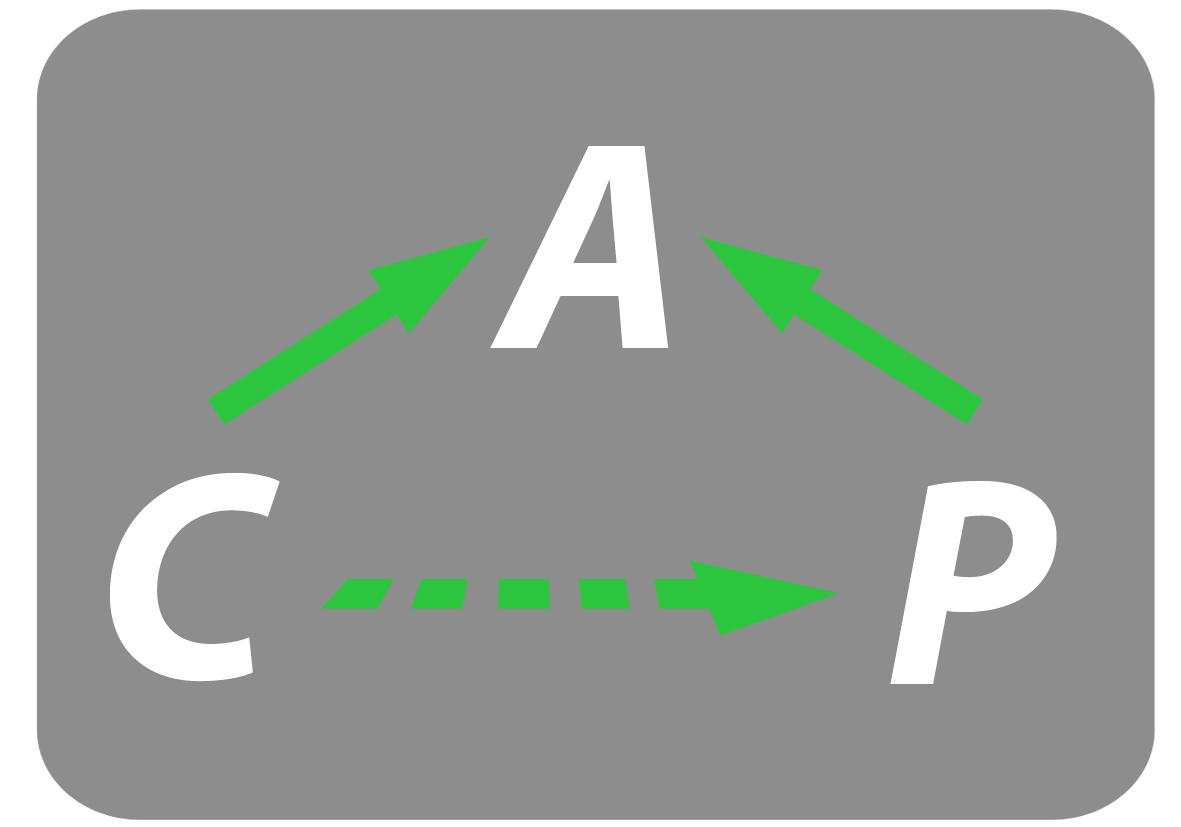
\includegraphics[width=\blockwidth,height=\blockheight]{Logo_CAP.jpg}};
  \begin{center}
   \begin{tikzpicture}[node distance=0.7cm,scale=0.6, every node/.style={scale=0.6}]
    {
    \node (intrinsic)[boxpackage, fill=\myblue] {IntrinsicCategories};
    }
    {
    \node (attribute)[boxpackage, fill=\myblue, below of= intrinsic] {AttributeCategory};
    \node (linearalgebra) [boxpackage, below of=attribute, fill=\myblue] {LinearAlgebra};
    \node (complexes) [boxpackage, below of=linearalgebra, fill=\myblue] {ComplexesAndFilteredObjects};
    \node (genmor) [boxpackage, below of=complexes, fill=\myblue] {GeneralizedMorphisms};
    \node (modulepres) [boxpackage, below of=genmor, fill=\myblue] {ModulePresentations};
    \node (homalg) [boxpackage, right = of genmor, fill=\myblue] {HomologicalAlgebra};
    \draw[->,thick] (homalg) |- (complexes);
    \draw[->,thick] (homalg.west) |- (genmor);
    }
    {
    \node (cap) [below = of modulepres] {};
    \begin{scope}[on background layer]
    \node (captotal) at ($(cap)+(1,0)$) [opacity=.20] {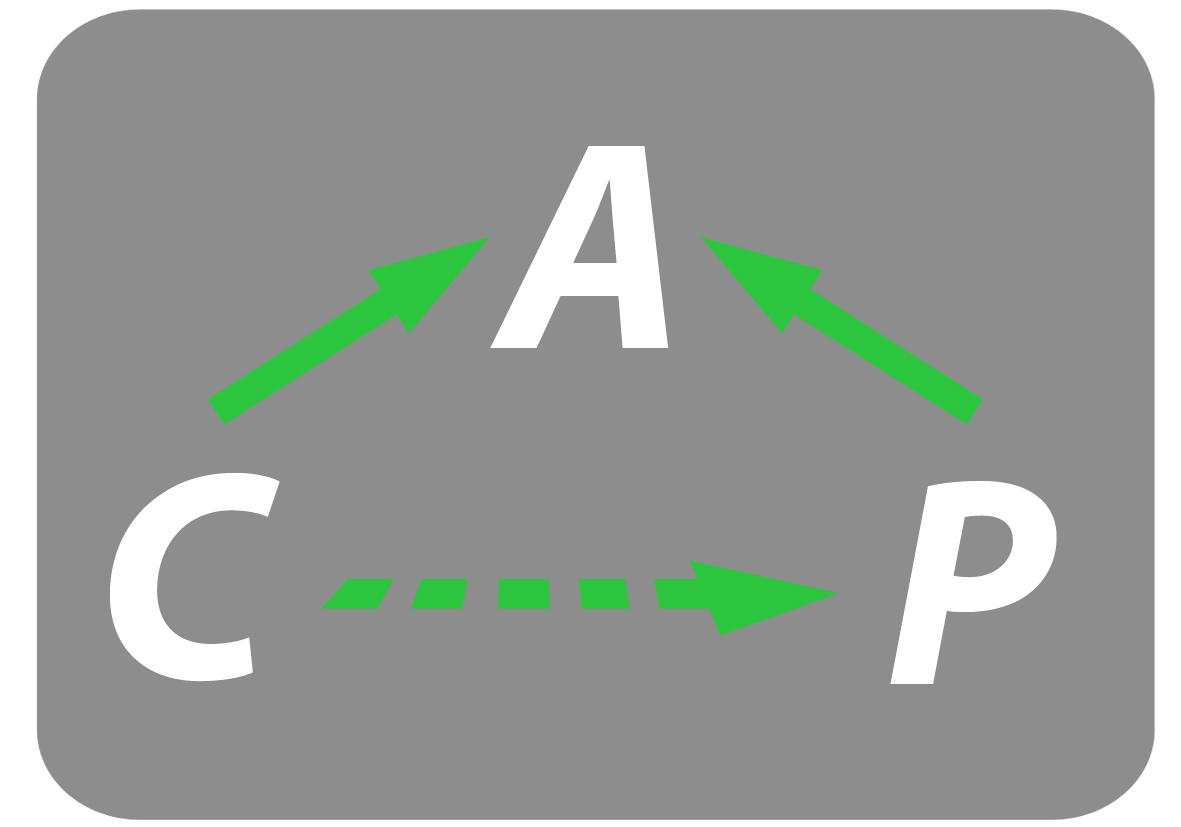
\includegraphics[width=1.4\textwidth]{Logo_CAP.jpg}};
    \end{scope}
    }
    
    {
    \node (ambient) [boxpackage, left = of attribute, fill=\myblue, xshift = -3em] {CategoriesWithAmbientObjects};
    \node (m2) [boxpackage, below = of ambient, fill=\myblue] {homalg2};
    \draw[->,thick] (m2) -- (ambient);
    \draw[->,thick] (m2) |- (modulepres);
    \draw[->,thick] (ambient) -- (attribute);
    }
    
    {
    \node (kamalcomplexes) [boxpackage, left = of cap, fill=\myblue, yshift = -4em] {complex};
    \node (stable) [boxpackage, below of=  kamalcomplexes, fill=\myblue] {StableCategories};
    \node (frobenius) [boxpackage, below of= stable, fill=\myblue] {FrobeniusCategories};
    \node (triangulated) [boxpackage, below of= frobenius, fill=\myblue] {TriangulatedCategories};
    \node (bicomplexes) [boxpackage, left= of kamalcomplexes, fill=\myblue] {Bicomplexes};
    \node (homotopy) [boxpackage, above= of bicomplexes, fill=\myblue, yshift = -2em, xshift = -1em] {HomotopyCategories};
    \draw[->,thick] (bicomplexes) -- (kamalcomplexes);
    \draw[->,thick] (homotopy.east) |- (kamalcomplexes);
    }
    
    {
    \node (qpa2) [boxpackage, right= of triangulated, fill=\myblue] {QPA2};
    }
    
    {
    \node (projectivegraded) [boxpackage, right = of cap, fill=\myblue, yshift = -4em] {CategoryOfProjectiveGradedObjects};
    \node (prescat) [boxpackage, below of = projectivegraded, fill=\myblue] {PresentationCategory};
    \node (presbyprojgraded) [boxpackage, below of = prescat, fill=\myblue, xshift = 8em] {PresentationsByProjectiveGradedModules};
    \draw[->,thick] (presbyprojgraded) |- (projectivegraded);
    \draw[->,thick] (presbyprojgraded) |- (prescat);
    }
    {
    \node (motives) [boxpackage, below = of m2, fill=\myblue, xshift = -3em] {MotivesForBiArrangements};
        }
    {
    \node (dmod) [boxpackage, right = of qpa2, fill=\myblue] {Bialgebroids};
    \draw[->,thick] (dmod) -- (qpa2);
    \node (functorcat) [boxpackage, below = of dmod, fill=\myblue] {FunctorCategories};
    \draw[->,thick] (functorcat) -- (dmod);
%     \node (bmod) [boxpackage, left = of functorcat, fill=\myblue,xshift=-1em] {BMod};
    }
    {
    \node (freydcats) [boxpackage, right = of dmod, fill=\myblue, yshift = -3em] {FreydCategories};
    \draw[->,thick] (freydcats) |- (dmod);
    }
    
    {
    \node (gradedmod) [boxpackage, right = of modulepres, fill=\myblue] {GradedModulePresentations};
    \node (toricsheaves) [boxpackage, below = of gradedmod, fill=\myblue] {ToricSheaves};
    \draw[->,thick] (gradedmod) -- (modulepres);
    \draw[->,thick] (toricsheaves) -- (gradedmod);
    }
    {
    \node (actions) [boxpackage, right = of attribute, fill=\myblue] {Actions};
    \node (groups) [boxpackage, right = of linearalgebra, fill=\myblue] {GroupRepresentations};
    \node (intext) [boxpackage, right = of groups, fill=\myblue] {InternalExteriorAlgebra};
    \draw[->,thick] (actions) -- (attribute);
    \draw[->,thick] (groups) -- (linearalgebra);
    \draw[->,thick] (intext) -- (groups);
    \draw[->,thick] (intext) |- (actions);
    \draw[->,thick] (intext) |- (complexes);
    }
    
    
    \end{tikzpicture}
  \end{center}
\end{frame}


% Connecting Homomorphism in the Snake Lemma

\begin{frame}[fragile]
 \frametitle{Snake lemma}

 \begin{block}{}
 \begin{center}
 \begin{tikzpicture}[mystyle/.style={scale=.7}]
  \matrix[matrix of math nodes,column sep={70pt,between origins},row sep={40pt,between origins}] (s)
  { & & & |[name=Kernel]| \kernel(\gamma) & \\
    &|[name=A]| A &|[name=B]| B &|[name=C]| C &|[name=01]| 0 \phantom{C}  \\
    |[name=02]| \phantom{a'} 0 &|[name=A']| A' &|[name=B']| B' &|[name=C']| C' \\
    & |[name=Coker]| \coker(\alpha) & & & \\
  };
              {\path[->,thick] (Kernel) edge node[mystyle,anchor=west] {} (C); }
              
              
              \path[->,thick] (C) edge (01);
              \path[->,thick] (A) edge (B);
              
              {\path[->,thick] (B) edge node[mystyle,anchor=south] {$\epsilon$} (C);}
              
              \path[->,thick] (A) edge node[mystyle,anchor=east] {$\alpha$} (A');
              
              {\path[->,thick] (B) edge node[mystyle, anchor=east] {$\beta$} (B');}
              
              \path[->,thick] (C) edge node[mystyle,anchor=east] {$\gamma$} (C');
              \path[->,thick] (02) edge (A');
              
              {\path[->,thick] (A') edge node[mystyle,anchor=north] {$\mu$} (B');}
              
              \path[->,thick] (B') edge (C');
              
              {\path[->,thick] (A') edge node[mystyle,anchor=east] {}(Coker);}
              \visible<2->{
              \draw[->,blue,rounded corners,thick] (Kernel) -| ($(01.east)+(.5,0)$) |- ($(B)!.35!(B')$) -|
    ($(02.west)+(-.5,0)$) |- (Coker);}
  \end{tikzpicture}
 \end{center}
 \end{block}
\end{frame}
